\documentclass[10pt]{article}
\usepackage{graphicx}
\usepackage{algorithm}
\usepackage{hyperref}
\usepackage{algorithmic}
\usepackage[margin=1.0in]{geometry}
\usepackage{float}
\usepackage{subcaption}
\usepackage{tikz}
\usetikzlibrary{shapes, arrows}


\parskip 0.05in
\begin{document}
\title{\bf Can we predict fire with weather data?}
\author{Harsh (hp444), Yi Yao (yy899), Murali (mt788)}
\maketitle

\begin{abstract}
\end{abstract}

\tableofcontents

\section{Introduction}
The weather has literally been the hot topic of discussion in recent times.
One aspect of weather data is that, when it is combined with other data
sets, it can be used to predict varied different aspects related to
the society. For example, one particular aspect could be how does traffic
conditions change based on the weather in a particular city or if there is
a correlation between crime rates and weather conditions. In this project,
we are trying to address a more important issue of predicting wildfires in
different cities based on weather conditions. Since the future weather data
is readily available these days, a good model would help predict these
wildfires in advance and take necessary precautions to completely avoid it.
This would help avoid human and wildlife loss. It would also help contain
the impact of these wildfires on the environment which increases the
content of poisonous gases in the environment, making the nearby
uninhabitable.\par
Wildfires are growing in frequency and intensity by the day. The 2019
wildfire season of California has more than 6800 fires recorded by the US
Forest Service and approximately 250000 acres of burnt land. These
wildfires could be the result of foul human activities but there has been
a lot of speculation on the high correlation of these fires with the
weather. Climate change is not only making the fire season longer but on
average much more intense. The idea is to use the model to predict these
fires in advance, thereby reducing such incidents.\par
\section{EDA}
\subsection{Covariates}
The features that we have in our Weather dataset are:
\begin{table}[H]
    \centering
    \caption{Covariates}
    \begin{tabular}{l|l|l}
        Covariate &Type &Description\\\hline
        Temperature & &\\
        Pressure & &\\
        Humidity & &\\
        Weather Description & &\\
        \textbf{Need to check} & &\\
    \end{tabular}
\end{table}
The features in the fire dataset is:
\begin{enumerate}
    \item erer
    \item erere
    \item erer4555
\end{enumerate}
\subsection{Basic Statistics}
The size of the dataset in the Fires table is: $number \times number$ and
the size in the weather table is: $1M \times 11$. The following figures
help illustrate what the dataset looks like\par
\begin{figure}[H]
    \centering
    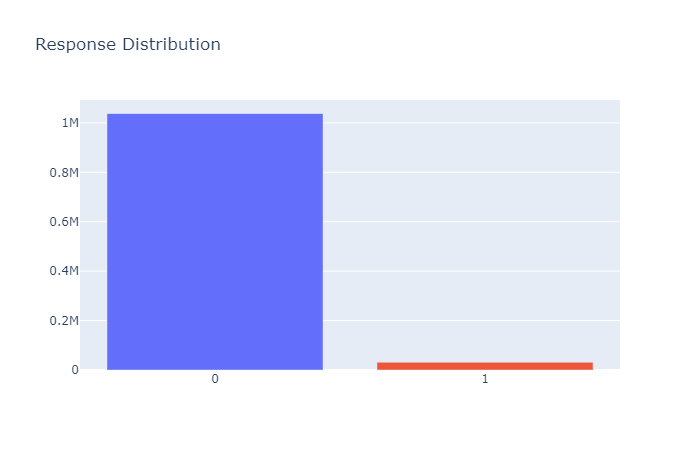
\includegraphics[width=0.5\textwidth]{../res/eda1.png}
    \caption{Response Distribution}
\end{figure}
\begin{figure}[H]
    \centering
    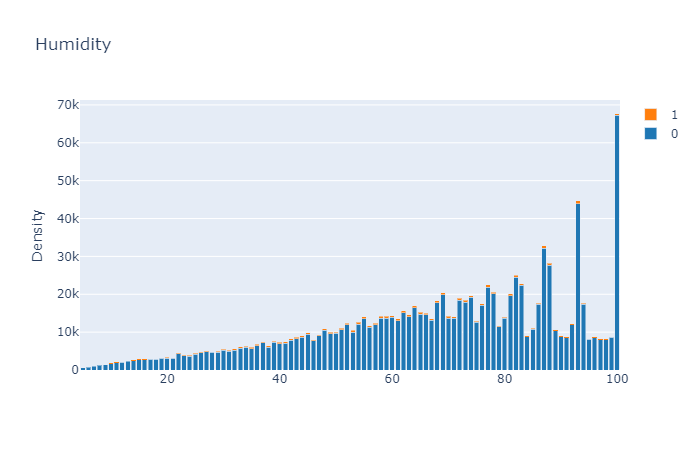
\includegraphics[width=0.5\textwidth]{../res/eda2.png}
    \caption{Histogram of Humidity}
\end{figure}
\begin{figure}[H]
    \centering
    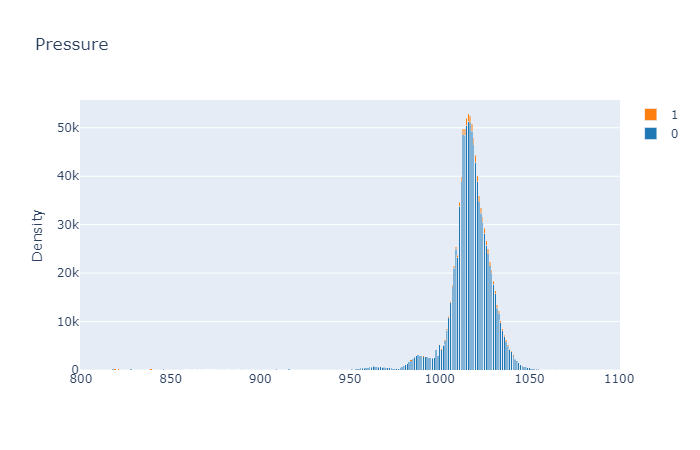
\includegraphics[width=0.5\textwidth]{../res/eda3.png}
    \caption{Histogram of Air Pressure}
\end{figure}
\begin{figure}[H]
    \centering
    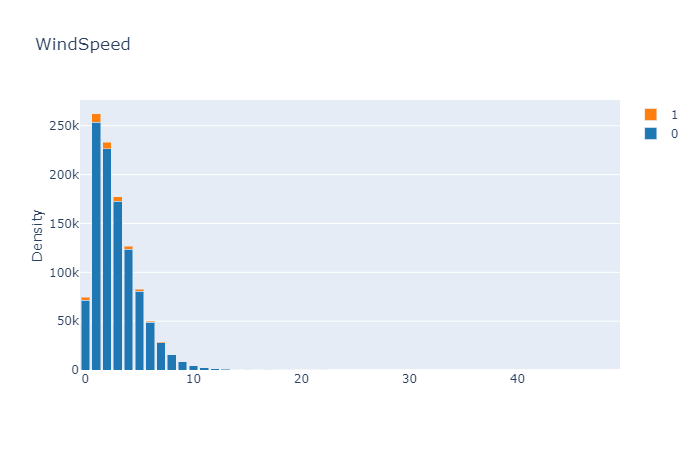
\includegraphics[width=0.5\textwidth]{../res/eda5.png}
    \caption{Histogram of Wind Speed}
\end{figure}
\begin{figure}[H]
    \centering
    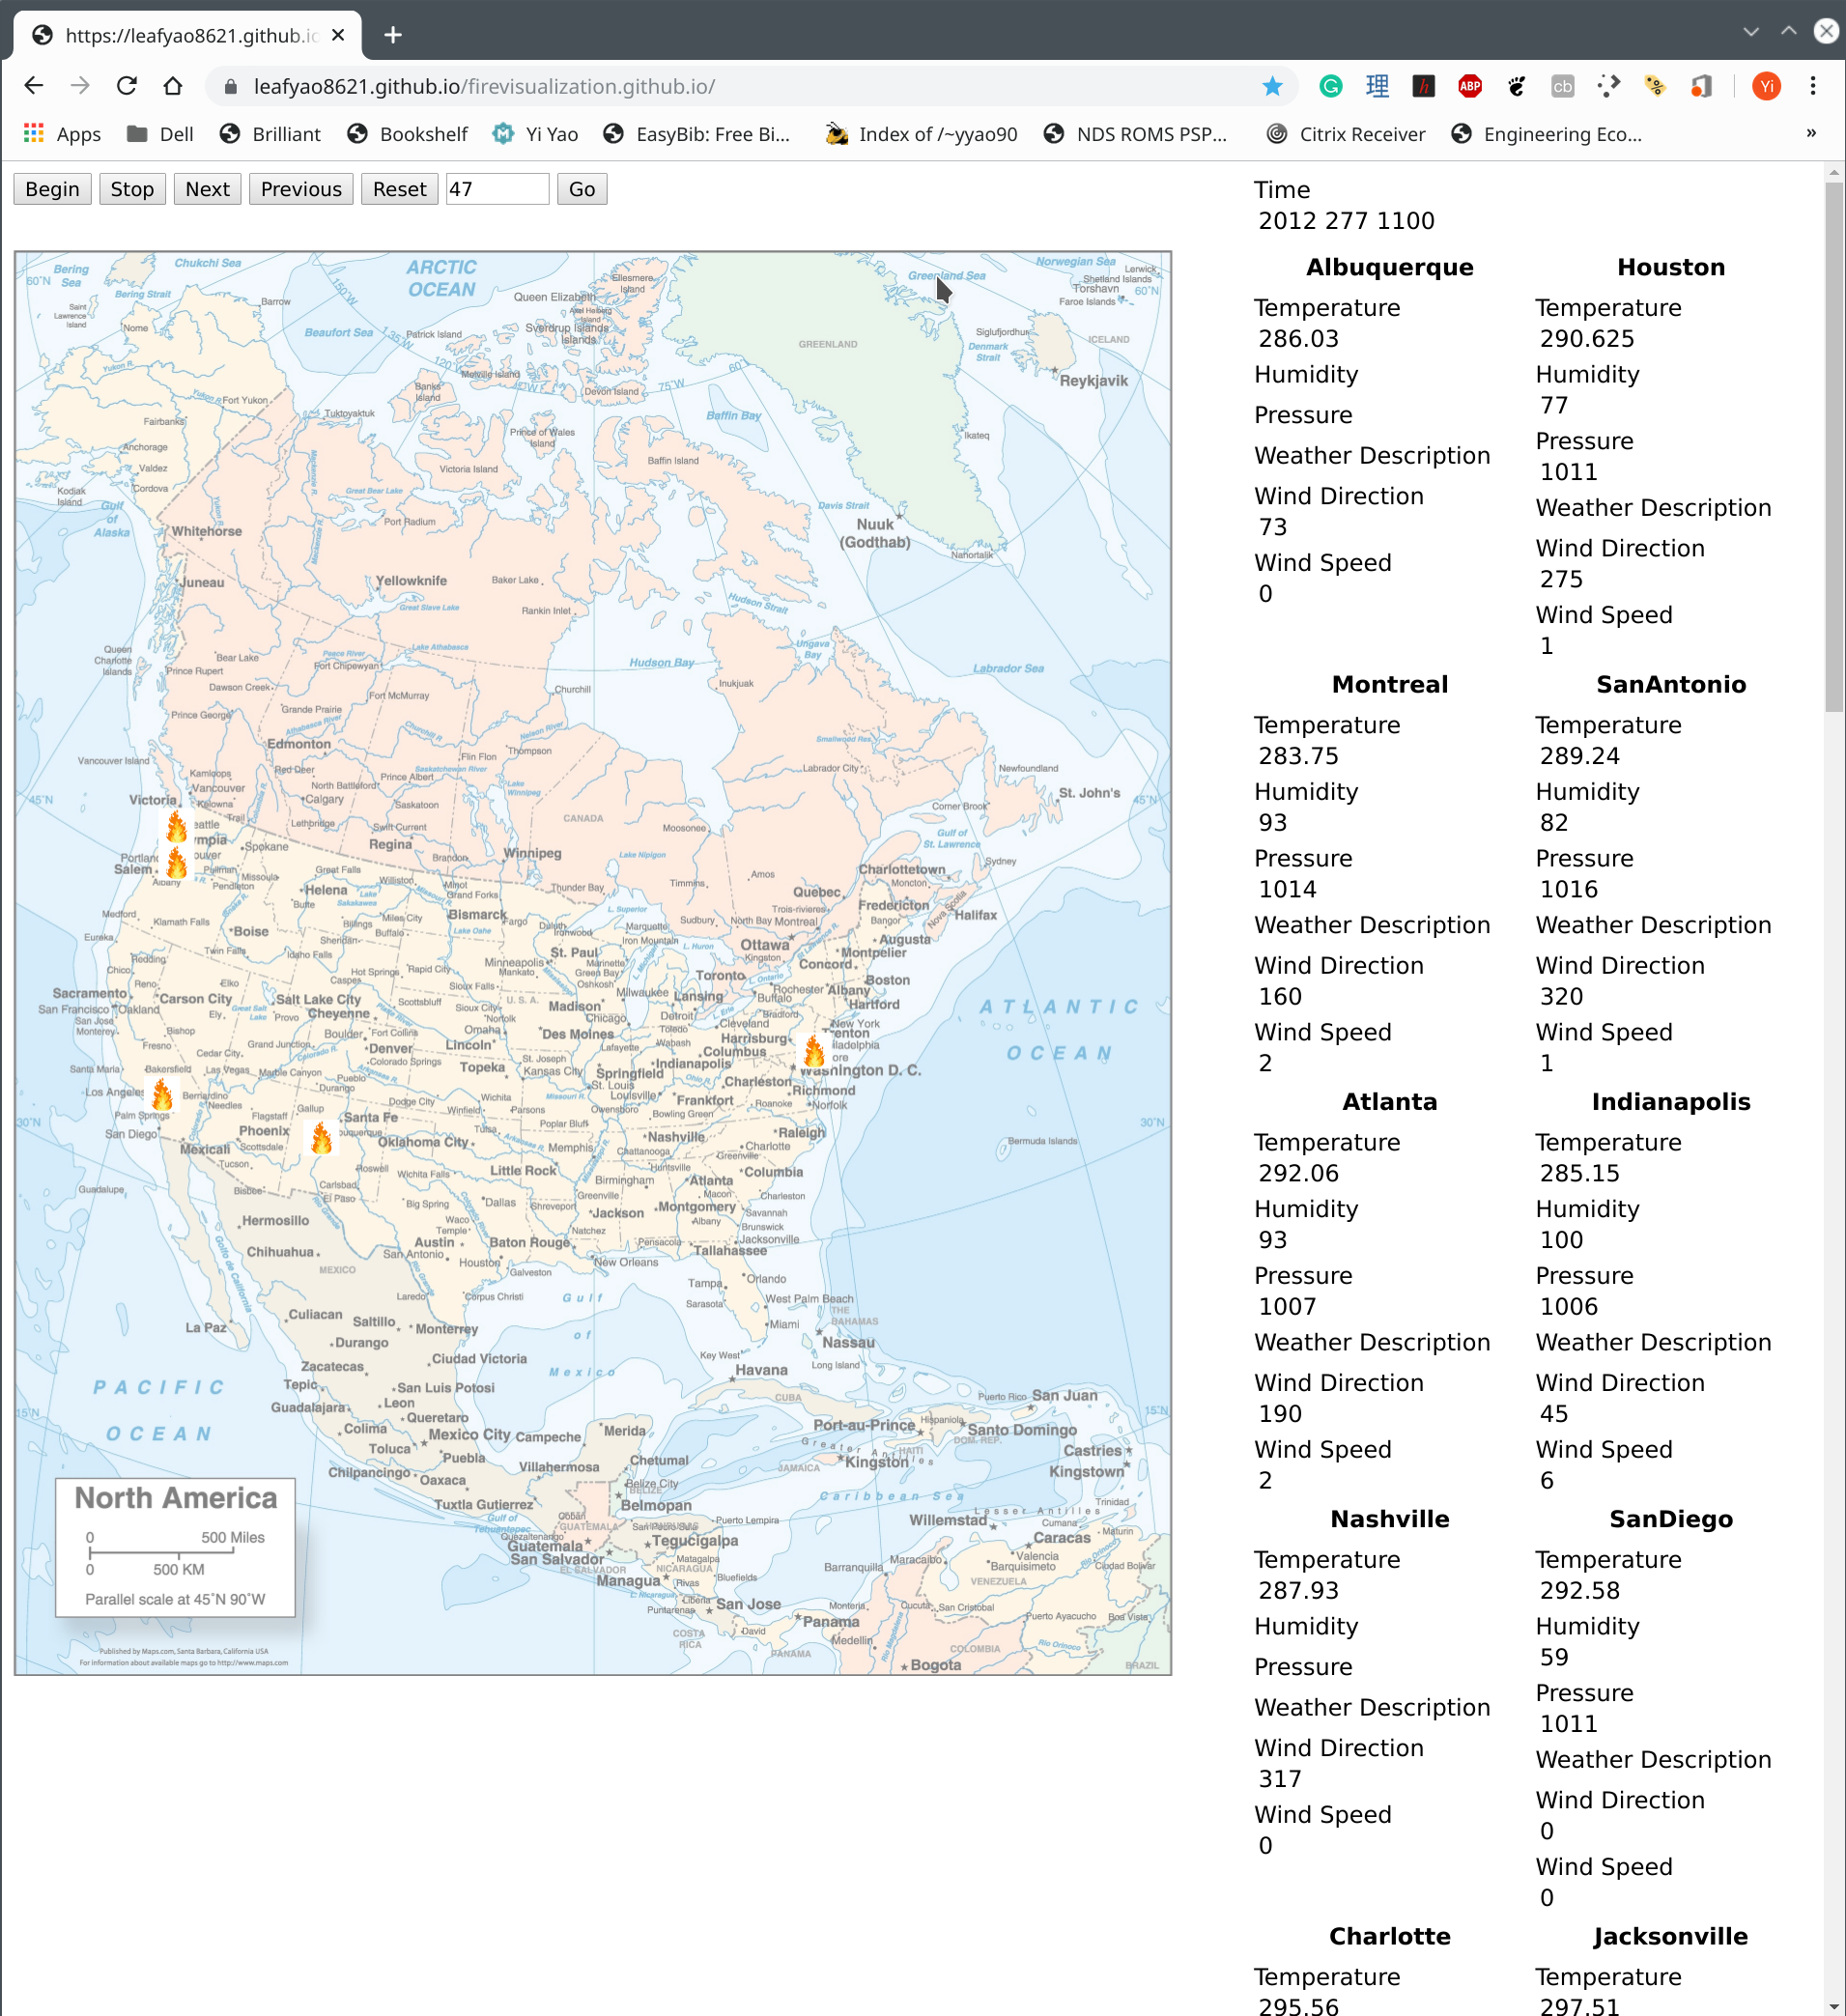
\includegraphics[width=0.5\textwidth]{../res/screenshot.png}
    \caption{Screenshot from Visualization Tool}
\end{figure}
\section{Model Building and Accuracy Tuning}
\begin{figure}[H]
    \centering
    \tikzstyle{block} = [rectangle, draw]
\tikzstyle{line} = [draw, -latex']
\begin{tikzpicture}
    \node [block] (n0)
    {$\begin{array}{l}
        \textbf{Experiment 0}\\
        \textrm{Random Forest}\\
        \textrm{XGBoost}\\
        \textrm{SVM with RBF Kernel}\\
        \textrm{Categorical Encoding}\\
    \end{array}$};
    \node [block, right of = n0, node distance = 55mm] (n1)
    {$\begin{array}{l}
        \textbf{Experiment 1}\\
        \textrm{Random Forest}\\
        \textrm{XGBoost}\\
        \textrm{SVM with RBF Kernel}\\
        \textrm{Balanced Under-sampling}\\
        \textrm{Categorical Encoding}\\
    \end{array}$};
    \node [block, below of = n1, node distance = 30mm] (n2)
    {$\begin{array}{l}
        \textbf{Experiment 2}\\
        \textrm{Boosted Random Forest}\\
        \textrm{Boosted XGBoost}\\
        \textrm{Balanced Under-sampling}\\
        \textrm{Categorical Encoding}\\
    \end{array}$};
    \node [block, left of = n2, node distance = 53mm] (n3)
    {$\begin{array}{l}
        \textbf{Experiment 3}\\
        \textrm{Random Forest}\\
        \textrm{XGBoost}\\
        \textrm{Balanced Under-sampling}\\
        \textrm{Boosting}\\
        \textrm{Ordinal Encoding}\\
    \end{array}$};
    \node [block, below of = n3, node distance = 35mm] (n4)
    {$\begin{array}{l}
        \textbf{Experiment 4}\\
        \textrm{Random Forest}\\
        \textrm{XGBoost}\\
        \textrm{Balanced Under-sampling}\\
        \textrm{Boosting}\\
        \textrm{Ordinal Encoding}\\
        \textrm{DBScan Clustering as Feature}\\
    \end{array}$};
    \node [block, right of = n4, node distance = 60mm] (n5)
    {$\begin{array}{l}
        \textbf{Experiment 5}\\
        \textrm{XGBoost}\\
        \textrm{SVM with RBF Kernel}\\
        \textrm{Decision Tree}\\
        \textrm{Stacked Ensemble}\\
        \textrm{Balanced Under-sampling}\\
        \textrm{Ordinal Encoding}\\
        \textrm{DBScan Clustering as Feature}\\
    \end{array}$};
    \path [line] (n0) -- (n1);
    \path [line] (n1) -- (n2);
    \path [line] (n2) -- (n3);
    \path [line] (n3) -- (n4);
    \path [line] (n4) -- (n5);
\end{tikzpicture}

    \caption{Flowchart of Experiments}
\end{figure}
\subsection{Preliminary Analysis}
\subsubsection{Primitive Model Fitting}
First, we fit XGBoost, Random Forest and SVM by using the entire dataset
and found the accuracy to be quite low. The low accuracy could be because
of the model overfitting. There are, afterall, 1M negative samples and
roughly 25k positive samples.\par
\subsubsection{Under-sampling}
Recognizing the unbalanced nature of our dataset, we created a balanced
training data set by combining all the positive samples with a random
subset of all the negative samples. Using this balanced training data set,
we fit XGBoost, Random Forest and SVM with RBF kernel. We observed a
significant improvement in test accuracy in the XGBoost and Random Forest
models; however, we have not observed any significant improvement in the
SVM models.\par
\subsection{Accurarcy Tuning}
\subsubsection{Boosting Models Fitted with Balanced Sub-samples}
Having the possibility of underfitting due to under-sampling in mind, we
have experimented with boosting to increase accuracy. By keeping all the
positive samples and randomly resampling negative samples equal to the
number of positive samples, we have kept the balance of the training data
set while making better use of the data set we have available.\par
\subsubsection{Clusters of Many-hot Encoding}
Having observed some order in the covariate ``Weather Description'', we
have experimented with many-hot encoding for ordinal variables. Since an
overall could not be established by the team, we have turned to many-hot
encoding on 3 clusters of levels and one-hot encoding on the remaining
levels. As for models, we continued to use the boosted algorithms in the
previous experiment.\par
\subsubsection{DBScan Clustering as Feature}
We have also experimented adding one-hot encoded output of an unsupervised
clustering algorithm, DBScan as covariates to the dataset to be fitted with
supervised models.
\subsubsection{Stacked Ensemble}
\subsubsection{Adding XGBoost to the Ensemble Model}

\section{Conclusion}
\end{document}
